\documentclass[10pt,oneside,slovak,a4paper]{article}

\usepackage[slovak]{babel}
\usepackage[IL2]{fontenc}
\usepackage[utf8]{inputenc}
\usepackage{graphicx}
\usepackage{url}
\usepackage{hyperref}
\usepackage{cite}

\pagestyle{headings}

\title{Path of Exile a role-playing games} 

\author{Mário Babiar\\[2pt]
	{\small Slovenská technická univerzita v Bratislave}\\
	{\small Fakulta informatiky a informačných technológií}\\
	{\small \texttt{xbabiar@stuba.sk}}
	}

\date{\small 11. októbra 2022}

\begin{document}
\maketitle

\begin{abstract}
Článok sa zameriava na hru Path of Exile (PoE) od vývojárskeho štúdia videohier Grinding Gear Games (GGG) a action role-playing hry (ARPG). 1) Vysvetľuje rôzne mechaniky v hre Path of Exile, jej históriu, charakteristické herné prvky a monetizáciu. 2) Porovnáva Path of Exile s inými hrami zo žánru ARPG/RPG, ako Diablo II alebo Diablo III. 3) Hodnotí v čom Path of Exile vyniká a prečo je jedna z najlepších hier vo svojom žánri, ale aj v čom zaostáva.\\\\
\end{abstract}
 
\section{Čo je Path of Exile}
Path of Exile je bezplatná online ARPG zasadená do temného sveta z názvom Wraeclast. Hra je silno inšpirovaná Diablo II a je často označovaná aj ako jeho nástupca. PoE je navrhnutá na základe silnej online ekonomiky, vytvárania výzbroje a hlbokého prispôsobenia postavy rôznymi spôsobmi. Hra je každé 3 mesiace obohacovaná novou expanziou nazývanou liga. Liga na konci roka v decembri alebo v januári je väčšia a je zameraná na rozšírenie konca hry a pridanie nových bossov.

\section{Grinding Gear Games}
Grinding Gear Games alebo GGG je vývojárske štúdio videohier založené v roku 2006 zo sídlom v Novom Zélande, ktoré vydalo iba jednu hru, a to Path of Exile. Medzí zakladateľov patria Chris Wilson (výkonný riaditeľ), Jonathan Rogers (technický riaditeľ), Erik Olofsson (Umelecký vedúci), Brian Weissman (Výkonný producent). Chris Wilson je výkonný riaditeľ a teda aj tvárou hry. Oznamuje každú novú expanziu do hry a pokiaľ prebieha nejaká Q\&A s vývojármi hry, tak práve Chris Wilson odpovedá na dané otázky.
\pagebreak

\section{Mechaniky v PoE}
\paragraph{Postavy}
Hráč má na výber zo 7 rôznych postáv. Každá postava začína na inej pozícii v pasívnom strome dôvodností, rôznymi atribútmi (sila, obratnosť, inteligencia) a odmenami z úloh od NPC (nehráčska postava). Neskôr v hre má každá postava na výber 3 rôzne podtriedy označované ako Ascendancy podtriedy.\cite{PoE-offisite-classes}

\paragraph{Pasívny Strom dovedností}
Je to rozsiahla sieť 1325 zručností, ktoré poskytujú pasívne bonusy postave. Za každé navýšenie úrovne postavy alebo splnenie niektorých úloh môžete prideliť ďalšie body do stromu. Popri bežných pasívnych schopností sa nachádzajú aj tzv. Notable a Keystone. Notable majú väčšie ikony, špecifické mena a väčšie efekty. Pomáhajú viesť hráčov pri budovaní postáv, tak že na prvý pohľad vidia čo skupina zručností okolo Notable ponúka. Keystone schopnosti však zásadne menia spôsob akým sa postava hrá. Zvyčajne majú jeden pozitívny účinok a jeden negatívny účinok. Napríklad Glancing Blows navýši šancu na blokovanie útoku alebo kúzla dvojnásobne, ale hráč utrpí 65\% poškodenia pokiaľ zablokuje útok alebo kúzlo.
\begin{figure*}[tbh]
\centering
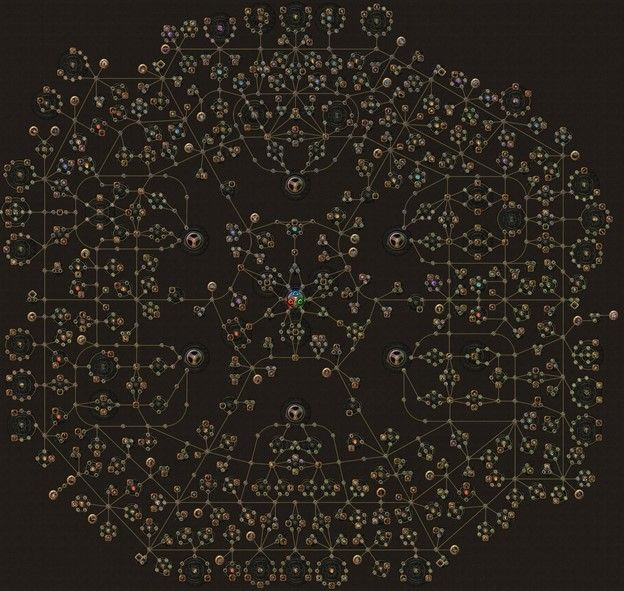
\includegraphics[scale=0.5,]{Path-of-exile-skill-tree.jpg}
\caption{Strom dovedností}\cite{PoE-skilltree}
\label{f:Strom dovedností}
\end{figure*}

%\paragraph{Ascendancy}

%\paragraph{Výzbroj}

%\paragraph{Skill Gems}

%\paragraph{Akty}

%\paragraph{Ligy}

%\paragraph{Koniec hry - Atlas}

%\section{Trading}

%\section{Ekonómia}

\section{Monetizácia}
Path of Exile je zadarmo (free-to-play) hra, napriek tomu sa v komunite často vyskytuje pojem ako zaplatiť za výhru (pay-to-win). V hre existujú 3 typy mikrotransakcií, kozmetické (úprava vzhľadu postavy, upráva vzhľadov efektov kúziel alebo útokov ap.), rozšírenie úložného priestoru a balík podporovateľa, ktorý obsahuje prémiovú menu a predovšetkým exkluzívne kozmetické veci. Pay-to-win pojem sa spája práve s rozšírením úložného priestoru, a preto by som sa na túto tému chcel zamerať trochu viac.\\

Hráč ma k dispozícii inventár (5x12 políčok) a externý úložný priestor označovaný ako truhla. V truhle sa nachádzajú záložky a každá má 12x12 políčok na uloženie vecí. Každý hráč má na začiatku hry 3 takéto záložky. Jediný spôsob ako získať viac záložiek je ich kúpou za reálnu menu. Existujú aj špeciálne záložky s rôznou cenou od 4\$ do 15\$\cite{PoE-shop-stash-tabs}, ktoré majú viac priestoru a špeciálne funkcie na uľahčenie manažmentu inventára.\\

Napríklad záložka na mapy ktorá stojí 15\$ umožňuje uložiť každý typ mapy rôznych úrovní 72-krát. Na úrovni 16 je 96 rôznych máp, teda je možné uložiť až 6912 máp iba pre túto jednu úroveň. Namiesto normálnej záložky, ktorá je neprehľadná a má maximum 144 políčok, resp. máp na uloženie je možné, aby si hráč kúpil špeciálny typ záložky pre mapy, ktorá je veľmi prehľadná, má niekoľko násobne väčší priestor a má viacero špeciálnych funkcií, ako napríklad zvýraznenie mapy, ktorá ešte nebola dokončená. Takýchto špeciálnych záložiek existuje niekoľko a pokrývajú všetky typy vecí, ako meny, mapy, úlomky, lekvárové fľašky atď.\\

Dôvodom prečo sa v komunite objavuje pojem pay-to-win je, že niektoré špeciálne záložky je priam potrebné kúpiť, aby si hráč mohol naplno vychutnať hru v jej konečnej fáze, kde pre mnohých hráčov práve hra začína.\\

V štúdii Volitional Vanity(Singh Martinez, Mauricio \& Tang, Sini)\cite{Volitional-Vanity} uviedlo ako prvú kúpu záložku 6 z 9 ľudí prostredníctvom rozhovoru a 10 z 23 ľudí prostredníctvom prieskumu. Ako prvú kúpu balíka podporovateľa uviedlo 2 z 9 ľudí prostredníctvom rozhovoru a 10 z 23 ľudí prostredníctvom prieskumu. Balík podporovateľa obsahuje prémiovú menu, za ktorú za záložky dajú kúpiť a teda sa treba pozrieť na následné kúpy a čo bola ich motivácia. V tejto istej štúdii motiváciu ďalšej investície do hry uviedlo 19 z 23 ľudí práve záložky a 16 z 23 uviedlo podporu vývojárom.\\

Z tohto vidíme, že hráči kupujú hlavne záložky alebo balík podporovateľa a neskôr záložky za prémiovú menu získanú z balíka. Teda pre nových hráčov sú hlavnou motiváciou investovania do hry práve záložky, ktoré oproti normálnym záložkám ponúkajú oveľa väčší úložný priestor a veľa funkcií na uľahčenie manažovania inventára tzv. quality-of-life features.\\

Pay-to-win pojem sa v komunite vyskytuje práve preto, že tieto záložky ponúkajú obrovské výhody nielen v ľahšom manažovaní inventára, čo hráčovi umožní si hru viac vychutnať užije hru viac, ale hlavne v ušetrení času a pri predávaní veľkých kvantít typov vecí ako napr. fragmenty. Špeciálne záložky preto majú vplyv aj na to, ako rýchlo vie hráč zarobiť a teda sú označované ako pay-to-win mechanika.

%\section{Gambling v PoE}

%\section{V čom PoE vyniká}

%\section{V čom PoE zaostáva}

%\section{Záver}

\nocite{*}
\bibliographystyle{plain}
\bibliography{literatura}
\end{document}
